\documentclass[a4paper,english, 10pt, twoside]{article}
\usepackage[utf8]{inputenc}
\usepackage[T1]{fontenc}
\usepackage[english]{babel}
\usepackage{epsfig}
\usepackage{graphicx}
\usepackage{amsfonts, amssymb, amsmath}
\usepackage{listings}
\usepackage{float}
\usepackage[top=2cm, bottom=2cm, left=2cm, right=2cm]{geometry}

%opening
\title{Project 3, FYS4150}
\author{Fredrik E Pettersen\\ fredriep@student.matnat.uio.no}


\begin{document}

\maketitle

% \begin{abstract}
% 
% \end{abstract}

\section*{About the problem}
The task of this project is to compute, with increasing degree of cleverness, the six dimensional integral used to determine the 
ground state correlation energy between two electrons in a helium atom. We will start off with ``brute force'' Gauss Legendre 
quadrature, proceed to Gauss Laguerre quadrature, and finish off with Monte Carlo integration. We assume that the wave function 
of each electron can be modelled like the single-particle wave function of an electron in the hydrogen atom. The single-particle 
wave function for an electron i in the 1s state is given in terms of a dimensionless variable (we ommit normalization of the wave 
functions)
$$
\mathbf{r}_i = x_i\mathbf{e}_x + y_i\mathbf{e}_y + z_i\mathbf{e}_z
$$
as
\begin{align*}
 \psi_{l,s}(\mathbf{r}_i) = e^{-\alpha r_i}
\end{align*}
where $\alpha$ is a parameter and 
$$
r_i = \sqrt{x_i^2 + y_i^2 + z_i^2}
$$
In this project we will fix $\alpha = 2$ which should correspond to the charge of the Helium atom $Z = 2$.
The ansatz for the two-electron wave function is then given by the product of two one-electron wave funtions.
$$
\Psi(\mathbf{r}_1,\mathbf{r_2}) = \psi(\mathbf{r}_1)\psi(\mathbf{r_2}) = e^{-2\alpha(r_1+r_2)}
$$
The integral we need to solve is the quantum mechanical expectation value of the
correlation energy between two electrons which repel each other via the classical Coulomb
interaction, namely
$$
\langle\frac{1}{\left|\mathbf{r}_1-\mathbf{r}_2\right|}\rangle = \int\limits^\infty_{-\infty}\int\limits^\infty_{-\infty}
\frac{ e^{-\alpha r_i}}{\left|\mathbf{r}_1-\mathbf{r}_2\right|}d\mathbf{r}_1d\mathbf{r}_2
$$

\section*{The algorithm}
The principle algorithms of this project is Gaussian quadrature and Monte Carlo integration. 
What we are actually doing when we integrate a function by the use of the rectangle, trapezodial or Simpsons rule is to 
approximate the integrand with a Taylor polynomial of degree 0,1 and 2 respectively between the integration points. An obvious 
step forward from here is to approximate the entire function with a Taylor polynomial of degree N-1 for N integration points, 
but then we realize that Taylor polynomials are a bit crude. A larger step forward can be obtained by approximating the 
integrand with an orthogonal polynomial, such as Legendre polynomials.  
We begin with the approximation
\begin{align*}
I = \int\limits^b_a f(x)dx = \int\limits_a^b W(x)g(x)dx \simeq \sum\limits_{i=1}^N w_i g(x_i)
\end{align*}
Where $w_i$ are the integration weights and W(x) is the weight function determined by the choise of orthogonal polynomial we use to 
approximate the integrand (W(x) = 1 for Legendre ploynomials).
This is called a Gaussian quadrature formula if it integrates exactly all polynomials $p \in P_{2N-1}$. That is:
$$
\int\limits_a^bW(x)p(x)dx = \sum\limits_{i=1}^Nw_ip(x_i)
$$
Let us now approximate $g(x) \simeq P_{2N-1}(x)$ where $P_{2N-1}(x) = \mathcal{L}_N(x)P_{N-1}(x)+Q_{N-1}(x)$. 
$\mathcal{L}_{N}(x)$ is an orthogonal polynomial e.g. a Legendre polynomial. We remember that orthogonal polynomials have the 
property
$$
\int\limits_a^b\mathcal{L}_i(x)\mathcal{L}_j(x)dx = A\delta_{i,j}
$$
where $x\in[a,b]$ is determined by the specific polynomial (e.g $x\in[-1,1]$ for Legendre) and A is some orthogonality relation 
also determined by the specific polynomial ($A = \frac{2}{2i+1}$ for Legende). This means that we have the following
$$
\int\limits_a^bf(x)dx \simeq \int\limits_a^bP_{2N-1}(x)dx =\underbrace{\int\limits_a^b\mathcal{L}_N(x)P_{N-1}(x)}_{=0} + 
\int\limits_a^bQ_{N-1}(x)
$$
When we now extrapolate this to our numerics the integrals take the form of sums. To ensure that the term 
$\int\limits_a^b\mathcal{L}_N(x)P_{N-1}(x) = 0$ we evaluate our sums in the points $\mathcal{L}_N(x_i) = 0$. That is
$$
\int\limits_a^bf(x)dx \simeq \sum\limits_{i=1}^{N-1}P_{2N-1}(x_i)w_i = \sum\limits_{i=1}^{N-1}Q_{N-1}(x_i)w_i
$$
The integration weights are simply the wheight function W(x) evaluated in the integration points.\\
The most general way to do the Gaussian Quadrature is to use Legendre polynomials. What we end up having to do in order to 
evaluate our integral is to choose some number of integration points, and then calculate the integration points and weights. 
That is we need to calculate the zeros of a Legendre polynomial of degree N. We will also need to make a mapping from the 
original limits of our integral to the limits of Legendre polynomials, $x\in [-1,1]$. This is done by the function ``gauleg'' 
found in the resources for the course. What this function is first of all to make a mapping from the limits one gives as 
input to the Legendre limits of -1 and 1. \\
   xm = 0.5 * (x2 + x1);\\
   xl = 0.5 * (x2 - x1);\\
After constructing the Legendre polynomial of degree i evaluated at some point x (from the recurrance relation),
the function runs Newtons method to find its zeros starting out with an appriximation\\
  pp = n * (z * p1 - p2)/(z * z - 1.0);\\
  z1 = z;\\
  z  = z1 - p1/pp;\\
and stores this in the vector x after scaling it according to the limits xm and xl. The roots of a Legendre polynomial are 
symmetric, so we actually find two roots for every iteration in ``gauleg''. The integration weights are also calculated through\\
w(i-1) = 2.0 * xl/((1.0 - z * z) * pp * pp);\\
theese are of course also symmetric.\\

Having done the general ``brute force'' gaussian quadrature and gotten very unsatisfying results we notice that the approach of 
first cutting the integral off at $\pm \lambda$ and then mapping theese limits to $\pm 1$ for all the variables 
$x_1,y_1,z_1,x_2,y_2,z_2$ is a rather clumsy one. If we rewrite the integrand into spherical coordinates we can use the Gauss 
Laguerre quadrature for the radial part instead, seeing as this looks like a typical Gauss Laguerre case:
$$
x^{\alpha}e^{-x}
$$
The transformation is
\begin{align*}
\iint \frac{e^{-4(r_1+r_2)}}{\left|\mathbf{r}_1-\mathbf{r}_2\right|}d\mathbf{r}_1\mathbf{r}_2 = 
\idotsint \frac{e^{-4(\sqrt{x_1^2 + y_1^2 + z_1^2}+\sqrt{x_2^2 + y_2^2 + z_2^2})}}{\sqrt{(x_1-x_2)^2+(y_1-y_2)^2+(z_1-z_2)^2}}
dx_1dx_2dy_1dy_2dz_1dz_2\\
 = \idotsint\frac{r_1^2r_2^2\sin(\theta_1)\sin(\theta_2)e^{-4(r_1+r_2)}dr_1dr_2d\phi_1d\phi_2d\theta_1d\theta_2}
 {\sqrt{(r_1cos(\phi_1)sin(\theta_1)-r_2cos(\phi_2)sin(\theta_2))^2
 +(r_1sin(\phi_1)sin(\theta_1)-r_2sin(\phi_2)sin(\theta_2))^2+(r_1cos(\theta_1)-r_2cos(\theta_2))^2}}
\end{align*}
We now look only at the denominator without the square root
\begin{align*}
r_1^2(cos^2(\phi_1)sin^2(\theta_1)+sin^2(\phi_1)sin^2(\theta_1)+cos^2(\theta_1)) + \\
r_2^2(cos^2(\phi_2)sin^2(\theta_2)+sin^2(\phi_2)sin^2(\theta_2)+cos^2(\theta_2)) -\\
2r_1r_2(cos(\phi_1)cos(\phi_2)sin(\theta_1)sin(\theta_2) + sin(\phi_1)sin(\phi_2)sin(\theta_1)sin(\theta_2) + cos(\theta_1)cos(\theta_2)\\
= r_1^2 + r_2^2 -2r_1r_2(cos(\theta_1)cos(\theta_2)+sin(\theta_1)sin(\theta_2)cos(\phi_1 - \phi_2))\\
= r_1^2 + r_2^2 -r_1r_2(cos(\theta_1+\theta_2)(1-cos(\phi_1 - \phi_2))+cos(\theta_1-\theta_2)(1+cos(\phi_1 - \phi_2)))
\end{align*}
So in the end we are left with
\begin{align*}
\int\limits_0^{\infty}\int\limits_0^{\infty}\int\limits_0^{2\pi}\int\limits_0^{2\pi}\int\limits_0^{\pi}\int\limits_0^{\pi}
\frac{r_1^2r_2^2\sin(\theta_1)\sin(\theta_2)e^{-4(r_1+r_2)}dr_1dr_2d\phi_1d\phi_2d\theta_1d\theta_2}
{\sqrt{r_1^2 + r_2^2 -r_1r_2(cos(\theta_1+\theta_2)(1-cos(\phi_1 - \phi_2))+cos(\theta_1-\theta_2)(1+cos(\phi_1 - \phi_2)))}}
\end{align*}
I need to remark that I use this denominator only because I thought I could simplify the expression more than it allready was in 
the project text, and had allready implemented the change before I relised I was wrong. I did not however bother changing it back 
seeing as it was correct, and the chance of introducing typos was rather large.\\
Now, when we intruduce this expression to the Gauss Laguerre quadrature both the $r_1^2r_2^2$ terms and the exponential will be 
baked into the wheight function if we do another small substitution $\rho_1 = 4r_1, \rho_2 = 4r_2$. This substitution will only 
introduce a factor $\frac{1}{1024}$ from inserting $r_i = \frac{\rho_i}{4}$ for all $r_i$ 
$$
\frac{\frac{\rho_1^2\rho_2^2}{4^24^2}sin(\theta_1)sin(\theta_2)e^{-(\rho_1+\rho_2)}\frac{d\rho_1d\rho_2}{4^2}}
{\sqrt{\frac{\rho_1^2}{4^2}+\frac{\rho_2^2}{4^2}-\frac{2\rho_1\rho_2}{4^2}cos(\beta)}} = 
\frac{\frac{1}{4^6}}{\frac{1}{4}}\frac{\rho_1^2\rho_2^2sin(\theta_1)sin(\theta_2)e^{-(\rho_1+\rho_2)}d\rho_1d\rho_2}
{\sqrt{\rho_1^2+\rho_2^2-2\rho_1\rho_2cos(\beta)}}
$$
This clearly results in 
$$
\frac{4}{4^6} = \frac{1}{1024}
$$
Finally we have an expression to send through our six nested for-loops. The Integration points and wheights are now determined 
by the Gauss Laguerre and Gauss Legendre for the radial and angular parts respectively.\\ \\

We do the Monte Carlo simulations in two different ways. The first is a brute force approach where we draw random points for the 
variables $r_1, r_2, \theta_1 , \theta_2 , \phi_1$ and $\phi_2$ in their respective intervals. We then evaluate 
$f(r_1, r_2, \theta_1 , \theta_2 , \phi_1, \phi_2)$ and calculate the mean of $f$ in the area $r_1,r_2 \in [0,\lambda]$, 
$\theta_1,\theta_2 \in [0,\pi]$, $\phi_1,\phi2 \in [0,2\pi]$ and multiply the mean of $f$ with the ``volume'' $V = 4\pi^4\lambda^2$
The reason we evaluate $f$ in spherical coordinates is that we only have to make cutoffs for the upper limits of $r_1$ and $r_2$, 
that is we limit ourselves to $r_1,r_2 \in [0,\lambda]$ when $r_1,r_2 \in [0,\infty)$ is correct. Had we evaluated $f$ in cartesian 
coordinates we would have had to make similar cutoffs for all the variables in both ends.\\
To get a measure of how good the appriximation is we calculate the variance and standard deviation of the result (we neglect the 
covaraiance because it is a heavy computation and because it is assumed to be small).

Next we think a little about what the function $f$ looks like, and realize that we can do importance sampling if we draw numbers 
from the exponential distribution. The integrand is then changed into
$$
\frac{1}{1024}\frac{\rho_1^2\rho_2^2\sin(\theta_1)\sin(\theta_2)}{\sqrt{\rho_1^2 + \rho_2^2 -2\rho_1\rho_2\cos(\beta)}}
$$
And in stead of just drawing our random numbers from the uniform distribution we want random numbers from a distribution on the 
form we see in equation \eqref{eq1}
\begin{equation}\label{eq1}
y = \int\limits_0^xe^{-x'}dx' = \left[-e^{-x'}\right]_0^x = 1-e^{-x}
\end{equation}
By some manipulation we find that we can achieve this by drawing a random number, y, from the uniform distribution, and set 
$$
x = -\ln(1-y)
$$
We are of course only interested in doing this for the radial parts of the integrand. The angular parts are treated in the same 
way as in the brute force Monte Carlo method, and agian they give us a factor of $4\pi^4$ which we need to account for in the 
final result.\\

In both of the Monte Carlo methods we use the variance and standard deviation as a measure of how accurate our results are. The 
variance is given by
\begin{equation*}
VAR(f) = \sigma^2_f = \langle f^2\rangle - \langle f \rangle^2 = \sum\limits_{i=1}^{N-1}f^2_i(r_1,r_2,\theta_1\theta_2,\phi_1\phi_2)
- \left(\sum\limits_{i=1}^{N-1}f_i(r_1,r_2,\theta_1\theta_2,\phi_1\phi_2)\right)^2
\end{equation*}
and the standard deviation is simply the sqare root of the variance
\section*{Analytic solution}
It is possible to find a closed form solution to the relevant integral, and put shortly it is$\frac{5\pi^2}{16^2}$.\\
With some help from David J Griffiths we can find this value ourselves to verify that it is correct.
We start out with
$$
\int\frac{e^{-4(r_1+r_2)/a}}{\left|\mathbf{r}_1 - \mathbf{r}_2\right|}d\mathbf{r}_1d\mathbf{r}_2
$$
where $a=1$ in our case. We will now fix $\mathbf{r}_1$ so we can do the $\mathbf{r}_2$ integral first. We also orient the 
$\mathbf{r}_2$ coordinate system such that the polar axis lies along $\mathbf{r}_1$. This gives us
$$
\left|\mathbf{r}_1 - \mathbf{r}_2\right| = \sqrt{r_1^2+r_2^2 -2r_1r_2cos(\theta_2)}
$$
which inserted gives
$$
I_{r_2} = \int\frac{e^{-4r_2}}{\sqrt{r_1^2+r_2^2 -2r_1r_2cos(\theta_2)}}d\mathbf{r}_2 = 
\int\frac{r_2^2sin(\theta_2)e^{-4r_2}}{\sqrt{r_1^2+r_2^2 -2r_1r_2cos(\theta_2)}}dr_2d\theta_2d\phi_2
$$
The integral over $\phi_2$ is trivial and ammounts to $2\pi$. The $\theta_2$ integral is
\begin{align*}
\int\limits_0^\pi\frac{sin(\theta_2)d\theta_2}{\sqrt{r_1^2+r_2^2 -2r_1r_2cos(\theta_2)}} 
= \frac{\sqrt{r_1^2+r_2^2 -2r_1r_2cos(\theta_2)}}{r_1r_2}\Bigg|_0^\pi\\
=\frac{1}{r_1r_2}\left(\sqrt{r_1^2 + r_2^2 +2r_1r_2}-\sqrt{r_1^2+r_2^2 -r_1r_2}\right)\\
=\frac{1}{r_1r_2}[(r_1+r_2)-\left|r_1-r_2\right|] = 
\begin{cases}
\frac{2}{r_1} \text{, if  } r_2<r_1 \\
\frac{2}{r_2} \text{, if  } r_1<r_2
\end{cases}
\end{align*}
Which means that
\begin{align*}
I_2 = 4\pi\left(\frac{1}{r_1}\int\limits_0^{r_1}e^{-4r_2}r_2^2dr_2 + \int\limits_{r_1}^\infty e^{-4r_2}r_2dr_2\right) = 
\frac{\pi}{8r_1}\left[1-\left(1+2r_1\right)e^{-4r_1}\right]
\end{align*}
And we can now do the integral over $r_1$
\begin{align*}
I = \frac{\pi}{8}\int\limits_0^\infty\int\limits_0^\pi\int\limits_0^{2\pi}
\left[1-\left(1+2r_1\right)e^{-4r_1}\right]e^{-4r_1}r_1sin(\theta_1)dr_1d\theta_1\phi_1
\end{align*}
The angular integrals are again trivial, and ammount to $4\pi$, giving us the final integral for $r_1$ (called r)
\begin{align*}
 I = \frac{\pi^2}{2}\int\limits_0^\infty\left[\underbrace{re^{-4r}}_{=\frac{1}{16}}-
 \underbrace{\left(r+2r^2)e^{-8r}\right)}_{=\frac{3}{128}}\right]dr = \frac{\pi^2}{2}\cdot\frac{5}{128} = \frac{5\pi^2}{16^2} 
 \simeq 0.19276571
\end{align*}
And there we have it. 
\section*{Results}
The quality of the results in this project of course depends on how close we get to the analytic solution derived in that section. 
Both in the case of Gaussian Quadrature and when we do Monte Carlo simulation the quality of our results are dependent on the number 
of integration points we can afford to use. For the Gaussian Quadrature we can see the results of increasing the number of 
integration points in table \ref{table1}. What we imediately can see from theese results is that the change to spherical coordinates 
and Gauss Laguerre quadrature has paid off. Not only does it give more accurate results for fewer integration poits, it also 
gives a more predictable convergence towards the correct result (as we can see in figure \ref{figure2})
\begin{figure}[H]
\centering 
\begin{tabular}{|c|c|c|c|}
\hline
N &Gauss Legendre &Gauss Laguerre & Correct result \\
\hline
10 & 0.0719797 & 0.186457 & 0.192765  \\
15 & 0.239088 & 0.189759 & 0.192765  \\
20 & 0.156139 & 0.191081 & 0.192765  \\
25 & 0.195817 & 0.19174 & 0.192765  \\
30 & 0.177283 & 0.192113 & 0.192765  \\
35 & 0.189923 & 0.192343 & 0.192765  \\
40 & 0.184417 & 0.192493 & 0.192765 \\
45 & 0.189586 & 0.192595 & 0.192765  \\
50 & 0.18756  & 0.192667 & 0.192765 \\
\hline
\end{tabular}
\caption{Results of Gaussian quadrature for increasing N}
\label{table1}
\end{figure}
\begin{figure}[H]
 \centering
 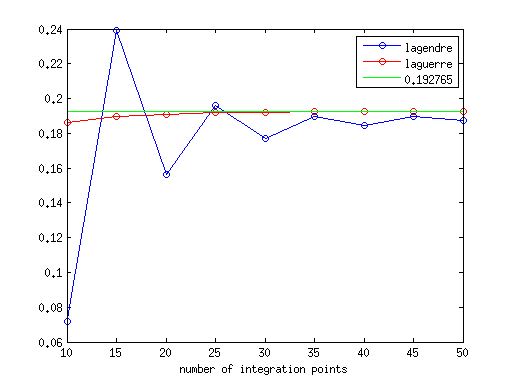
\includegraphics[scale=0.7]{convergence_quadrature.png}
 \caption{Results of integration by Gaussian Quadrature for increasing number of integration points}
 \label{figure2}
\end{figure}

What we have not said anything about yet is that the Gaussian Quadrature calculations recuire 6 nested for-loops, meaning $n^6$ 
FLOPS ($38n^6$). So there is a reason why figure \ref{table1} stops at $n = 50$. This calculation took close to 10 minutes, and increasing n 
further would therefore require a lot more CPU time.  As a comparison we can turn to table \ref{table2} where the results of the 
Monte Carlo simulations are listed. Notice in particular the CPU-time spent on theese calculations. Agreed, the Gaussian quadrature 
does give better results (or at least the Gauss Laguerre quadrature does) than the brute force approach, but we get a pretty decent 
result even from this crude approach using one tenth of the CPU-time. Compared to the brute fore Gaussian Quadrature, even the 
brute force Monte Carlo method is way better.
\begin{figure}[H]
\centering 
\begin{tabular}{|c|c|c|c|c|c|c|}
\hline
N &Brute force MC & time [ms] &$\sigma^2$&Imp. sampling & time [ms]&$\sigma^2$ \\
\hline
$10^3$ & 0.220502 & 0 & 1.08421e-07& 0.222254 & 2.5 & 1.19579e-05 \\
$10^4$ & 0.445336 & 0 &6.29848e-05& 0.314501 & 2.5 & 0.000248402  \\
$10^5$ & 0.377543 & 15 & 0.000357245& 0.200956 & 17.5 & 2.9042e-05 \\
$10^6$ & 0.212387 & 123 & 3.88044e-05& 0.192787 & 140 & 9.13831e-06 \\
$10^7$ & 0.196049 & 1170 & 4.64054e-06& 0.192867 & 1407 & 7.21355e-06 \\
$10^8$ & 0.194253 & 11700 & 5.68446e-05& 0.193275 & 14130 & 8.74453e-06 \\
$5\cdot10^8$ & 0.192253 & 58780 & 6.2599e-05& 0.194987 & 70690 & 0.00014808\\
\hline
\end{tabular}
\caption{Results for increasing number of Monte Carlo cycles using the ran0 random generator}
\label{table2}
\end{figure}

I would also like to mention the main results in speed up achieved from implementing paralellization through openmp. I ended up 
using openMP for two reasons; it was very easy to implement, and I don't know how to use MPI or openMPI yet and did not have the 
time to learn it properly. Luckily, we have the 
perfect case for testing the gain in speed in this project. The six nested for-loops from the quadrature calculations. As we can 
see from figure \ref{table3} the speed up is not quite as good as we could have hoped for seeing as there is no comminucation 
needed between the cores, but we still get a very noticable increace in speed. The reason that we do not see a ``perfect'' increace 
in computation speed is, I persume, that openMP is very easy to use. This is almost allways synonimus to large overhead, and 
complicated processes behind the curtains. It does, however look like the computations go something like 3 times faster using 
4 cores. 

\begin{figure}[H]
\centering 
\begin{tabular}{|c|c|c|c|}
\hline
N & time with 1 core & time with 2 cores & time with 4 cores \\
\hline
20 &  8000 ms & 4265 ms& 3112.5 ms\\
30 & 91 s & 52 s& 34.4 s \\
40 & ? & 284 s & 198 s  \\
\hline
\end{tabular}
\caption{Increase in computational speed when introducing more cores to do the Gauss Legendre quadrature calculations.}
\label{table3}
\end{figure}

\section*{Stability and precision}
The precision of Gausian quadrature is very dependent on how well the roots of the chosen orthogonal polynomial correspond with 
the varations of the function over the relevant area. The entire idea behind Gaussian Quadrature is to focus the integration 
points to the area where the integrand varies most, and to place fewer integration points where the integrand is small or varies 
slowly. This is the reason why we see the Gauss Legendre quadrature oscillate. For some values of N the roots of the Legendre 
polynomial correspond very well with the variations in the integrand, and for other values of N it doesn't.\\
This also explains why the Gauss Laguerre quadrature has (seemingly) an very good convergence. It already assumes an integrand on 
the form that we have, and thus the roots will always correspond quite well with where the integrand vaies the most.\\ \\

The stability of the Monte Carlo simulations depend on how random our random numbers are, how many Monte Carlo cycles 
we run, and where we end up pulling the random numbers from. As mentioned in the section regarding the algorithms we draw random 
numbers more or less within the correct intervals allready, but we could still get unlucky and dra a lot of points from an area 
which does not contribute much to the final result. This is also why the results of the Monte Carlo simulations vary for every time 
we run the program

\section*{Final comments}
Event though Gaussian Quadrature (especially with Laguerre polynomials) is an awesome approach to solving the integral, it just 
takes to much time to run it for as many as 6 dimensions (Pardon my somewhat unacademic language here, but I am truly amazed 
at how elegant this is).\\
I must say that I am not too impressed with the increace in performance when canging from brute force to importance sampled 
Monte Carlo methods. It looks like the importance sampled Monte Carlo method gives pretty good results between $N = 10^5 - 10^7$, 
but beyond that it only gets worse again. This can be seen from the variance in figure \ref{table2}. Around the relevand interval 
the importance sampled Monte Carlo method gives both better results and better (lower) variance, but outside of this interval I 
would say that the brute force method is at least as good.\\

\section*{Source code}
The source code is listed in full length in the appendix. I have also this time collected all of my functions in a header file for 
the same reasons as last time.
\end{document}

